\section{CQ1}

\begin{fancyquote}
    \textbf{CQ1a)} Find all NON Confirmable DELETE requests directed to the coap.me server that received a successful response. Take note of the MID of such requests.\\
    \textbf{CQ1b)} How many of the requests found in point CQ1a) actually obtained the desired outcome?
\end{fancyquote}

\vspace{0.3cm}

\noindent
\begin{minipage}{\linewidth}
\subsection{Find \textit{"coap.me"} IP address}
This can be done by looking up DNS requests:
\begin{lstlisting}
dns.qry.name == "coap.me" && dns.flags.response == 1
\end{lstlisting}
\vspace{-0.2cm}
\begin{figure}[H]
    \centering
    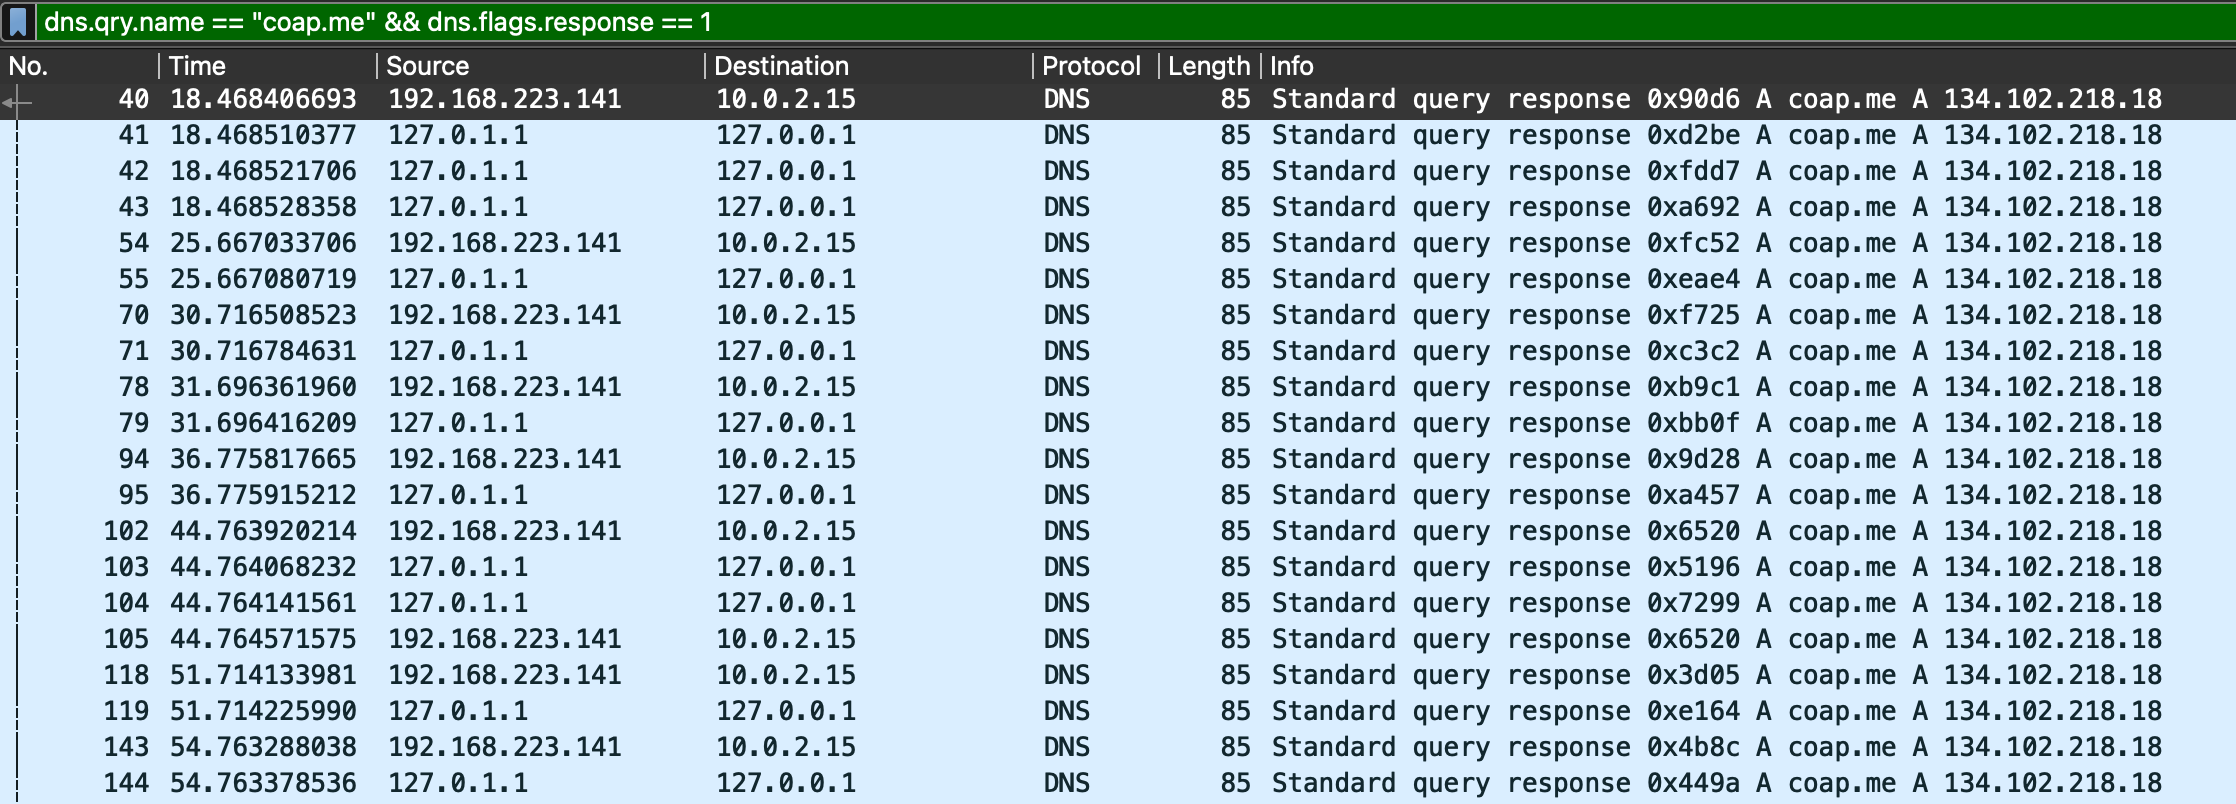
\includegraphics[width=0.9\linewidth]{images/coap_ip_wireshark.png}
\end{figure}
From these \textbf{DNS requests}, it is possible to retrieve the \textbf{coap.me} IP address: \textbf{134.102.218.18}.
\end{minipage}

\vspace{0.5cm}

\subsection{CQ1a - Find all NON Confirmable DELETE requests directed to the coap.me server that received a successful response. Take note of the MID of such requests}

Now 2 filters have to be used to identify if the request received a "successful response".

\begin{figure}[H]
    \centering
    \begin{minipage}[t]{0.48\textwidth}
        \textbf{Filter 1: Isolate NON DELETE Requests}
\begin{lstlisting}
ip.dst == 134.102.218.18 && coap.type == 1 && coap.code == 4
\end{lstlisting}
\begin{lstlisting}
tshark -r A.pcapng -Y "ip.dst == 134.102.218.18 && coap.type == 1 && coap.code == 4" -T fields -e coap.token -e coap.mid -e coap.opt.uri_path > non_deletes.txt
\end{lstlisting}

        First, we extract the Token, MID, and Uri-Path of all NON (type == 1) DELETE (code == 4) requests directed to the server.
        \vspace{0.2cm}
    \end{minipage}\hfill
    \begin{minipage}[t]{0.48\textwidth}
        \textbf{Filter 2: Isolate "2.02 Deleted" Responses}
\begin{lstlisting}
ip.src == 134.102.218.18 && coap.code == 66
\end{lstlisting}
\begin{lstlisting}
tshark -r A.pcapng -Y "ip.src == 134.102.218.18 && coap.code == 66" -T fields -e coap.token > 202_responses.txt
\end{lstlisting}
        We filter the traffic coming from the server for the specific 2.02 Deleted response (code == 66) and extract their Tokens.
        \vspace{0.2cm}
    \end{minipage}
\end{figure}

\noindent
\begin{minipage}{\linewidth}
The outputs of the two commands are saved in two files. To respond to question \textbf{CQ1a}, the two outputs are compared:

\begin{figure}[H]
    \centering
    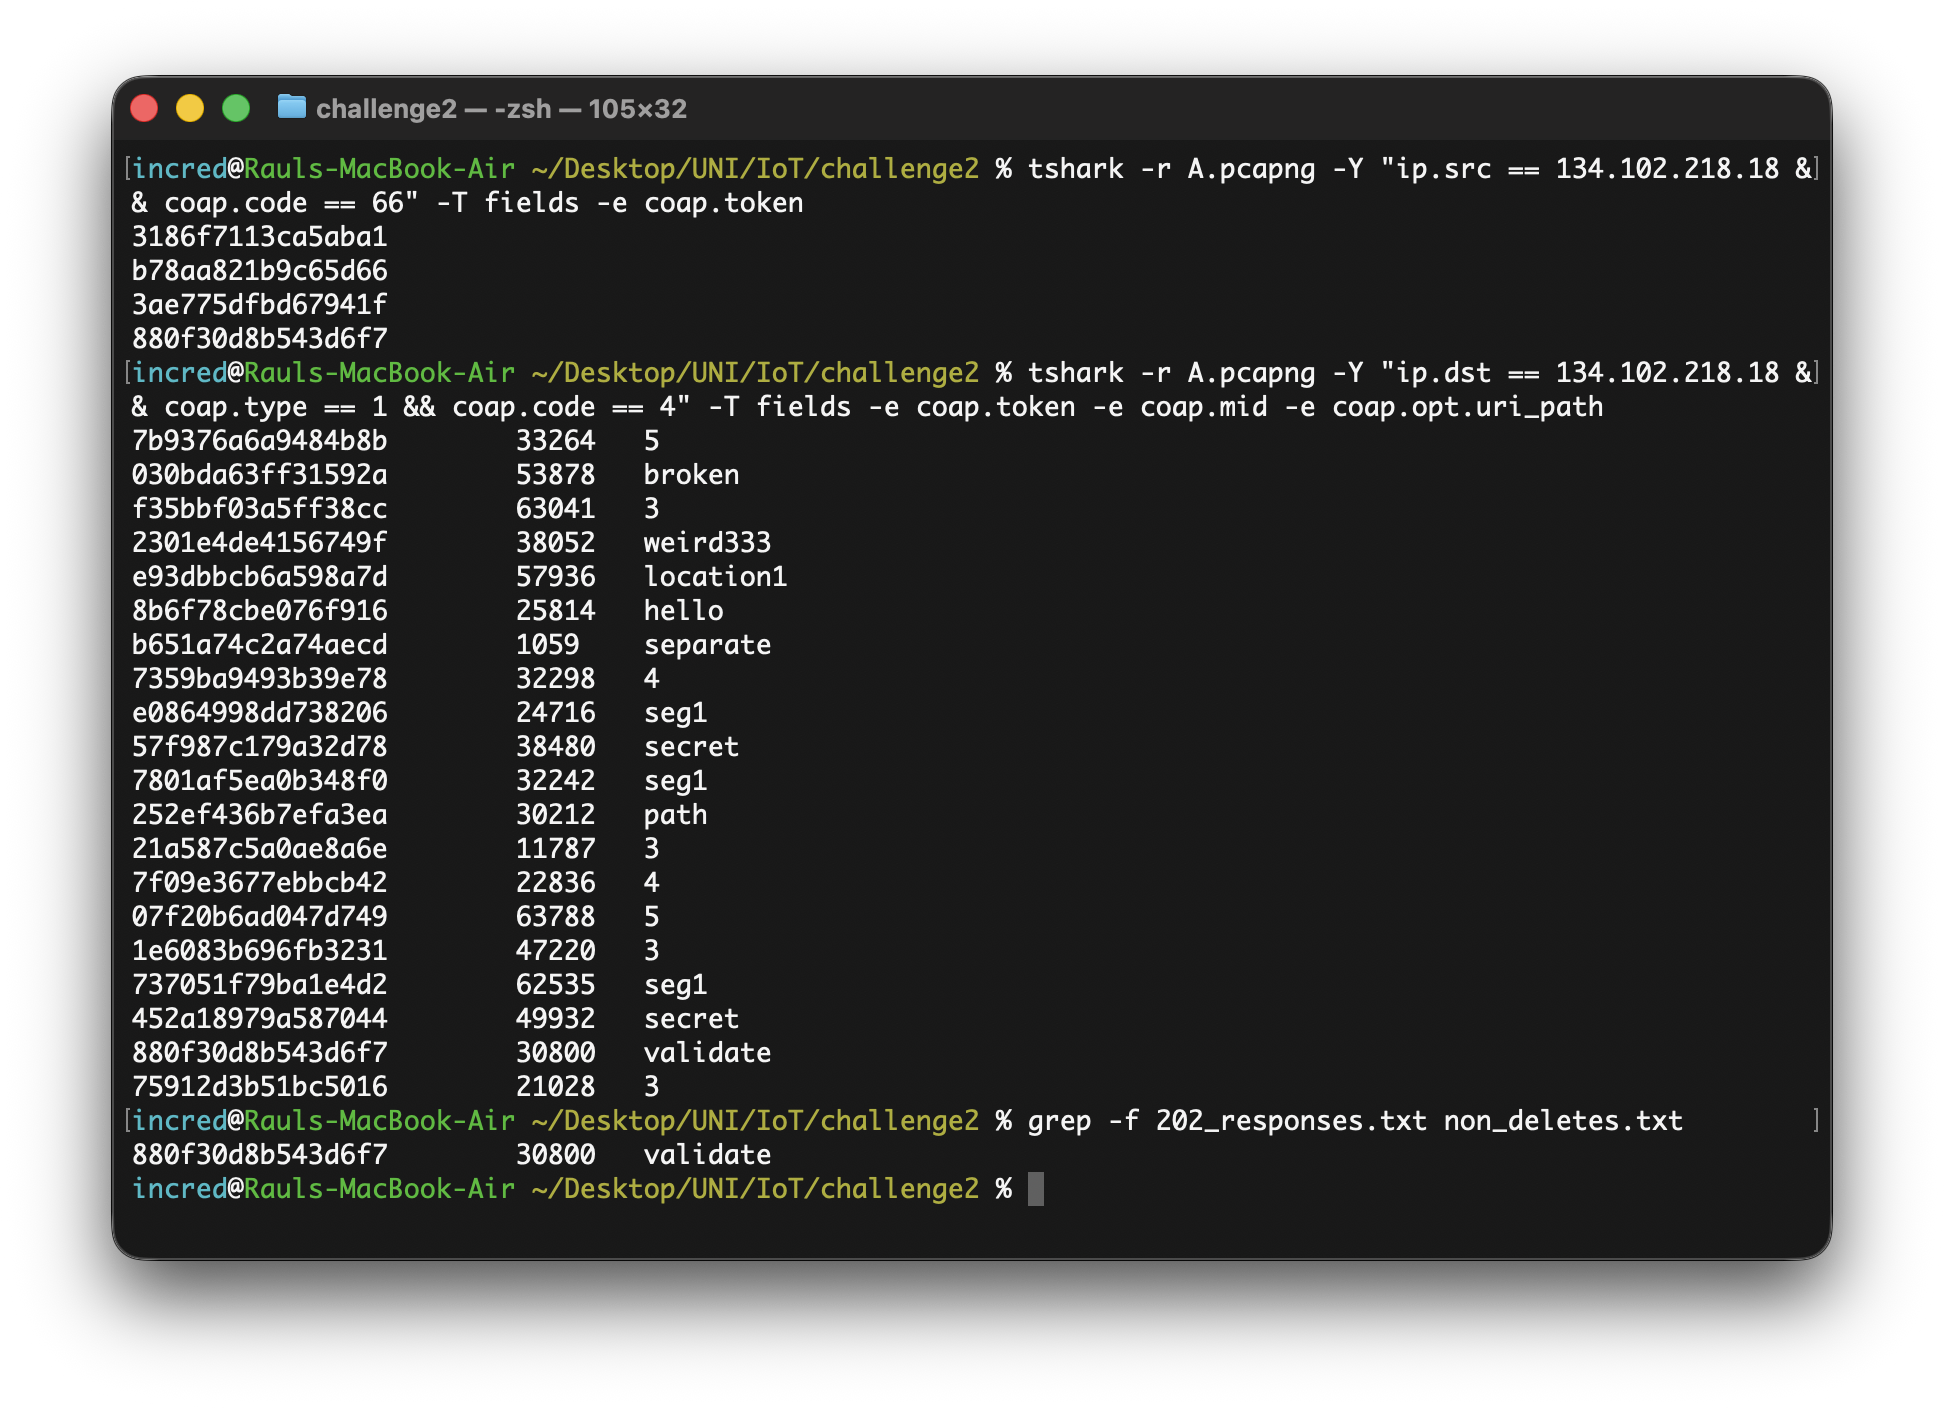
\includegraphics[width=0.65\linewidth]{images/cq1-result.png}
\end{figure}

By cross-referencing the Tokens from the successful responses against our initial list of requests, we isolate the DELETE requests that the server actively accepted.
\end{minipage}

\vspace{0.5cm}

\textbf{\huge Answer CQ1a: 30800}

\vspace{0.5cm}

\noindent
\begin{minipage}{\linewidth}
\subsection{CQ1b - How many of the requests found in point CQ1a) actually obtained the desired outcome?}
Receiving a \texttt{2.02 Deleted} response only confirms that the server \textit{accepted} the request. In IoT environments, this does not guarantee the resource was physically removed. To prove the desired outcome was achieved, it is necessary to observe the network traffic for a subsequent \texttt{GET} request directed to the exact same \texttt{Uri-Path}. If the deletion was truly successful, the server must respond to that new \texttt{GET} request with a \texttt{4.04 Not Found} (Code 132) error.

\subsubsection*{Extract the Deleted URIs}
Extract the \texttt{Uri-Path} (3rd column) from the successfully accepted DELETEs found in CQ1a.
\begin{lstlisting}[language=bash]
awk '{print $3}' accepted_deletes.txt > deleted_uris.txt
\end{lstlisting}
\end{minipage}

\vspace{0.3cm}

\noindent
\begin{minipage}{\linewidth}
\subsubsection*{Isolate All GET Requests}
Extract the Token and \texttt{Uri-Path} for all \texttt{GET} requests (\texttt{code == 1}) sent to the server.
\begin{lstlisting}[language=bash]
tshark -r A.pcapng -Y "ip.dst == 134.102.218.18 && coap.code == 1" -T fields -e coap.token -e coap.opt.uri_path > all_gets.txt
\end{lstlisting}
\end{minipage}

\vspace{0.3cm}

\noindent
\begin{minipage}{\linewidth}
\subsubsection*{Find GET Requests Targeting the Deleted URIs}
Cross-reference the list of deleted URIs against all GET requests to find attempts to access the deleted resources. The \texttt{-w} and \texttt{-F} flags force exact string matching to prevent false positives from hexadecimal substring overlaps.
\begin{lstlisting}[language=bash]
grep -w -F -f deleted_uris.txt all_gets.txt | awk '{print $1}' > get_tokens.txt
\end{lstlisting}


\vspace{0.3cm}

\noindent

\subsubsection*{Isolate "4.04 Not Found" Responses}
Extract the Tokens of all \texttt{4.04 Not Found} (\texttt{code == 132}) responses originating from the server.
\begin{lstlisting}[language=bash]
tshark -r A.pcapng -Y "ip.src == 134.102.218.18 && coap.code == 132" -T fields -e coap.token > 404_responses.txt
\end{lstlisting}


\vspace{0.3cm}

\noindent
\subsubsection*{Correlate to Prove Deletion}
Compare the Tokens of the \texttt{4.04} responses against the Tokens of the \texttt{GET} requests that targeted the deleted URIs. Piping the output to \texttt{wc -l} counts the exact number of verified deletions.
\begin{lstlisting}[language=bash]
grep -w -F -f 404_responses.txt get_tokens.txt | wc -l
\end{lstlisting}

\vspace{0.3cm}

\begin{figure}[H]
    \centering
    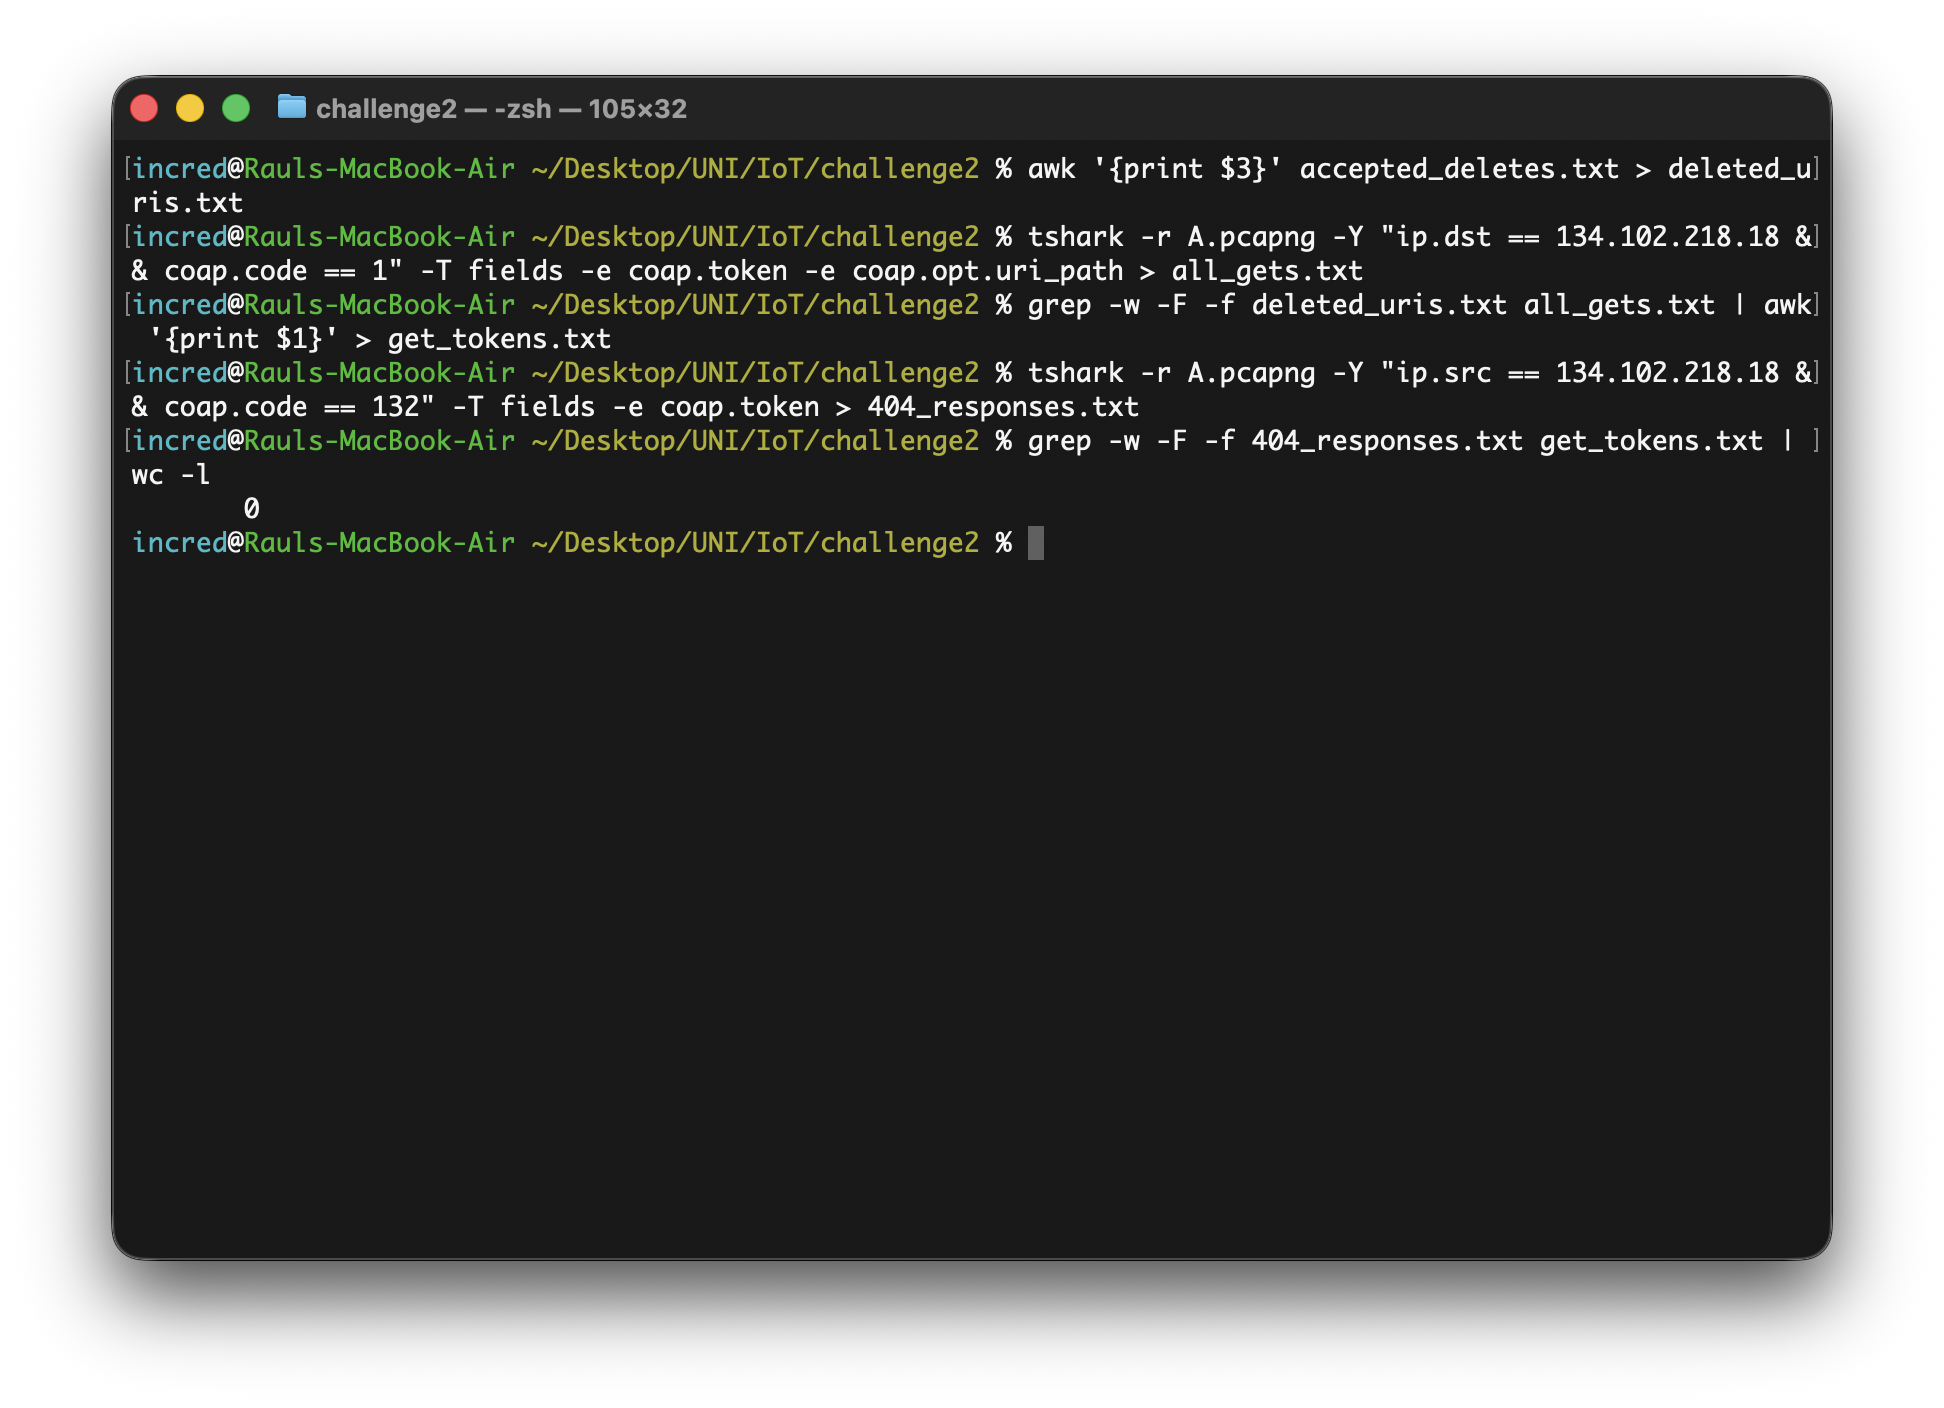
\includegraphics[width=0.7\linewidth]{images/cq1b-result.png}
\end{figure}

\textbf{\huge Answer CQ1b: 0}

\vspace{0.3cm}
\textit{Conclusion: The result of 0 proves that while the coap.me server politely accepted the DELETE commands (replying with 2.02), it did not actually delete the resources, as subsequent queries for those paths did not return a 4.04 Not Found.}
\end{minipage}